\documentclass{article}
\usepackage{tikz}
\usetikzlibrary{calc}

\begin{document}
\begin{center}
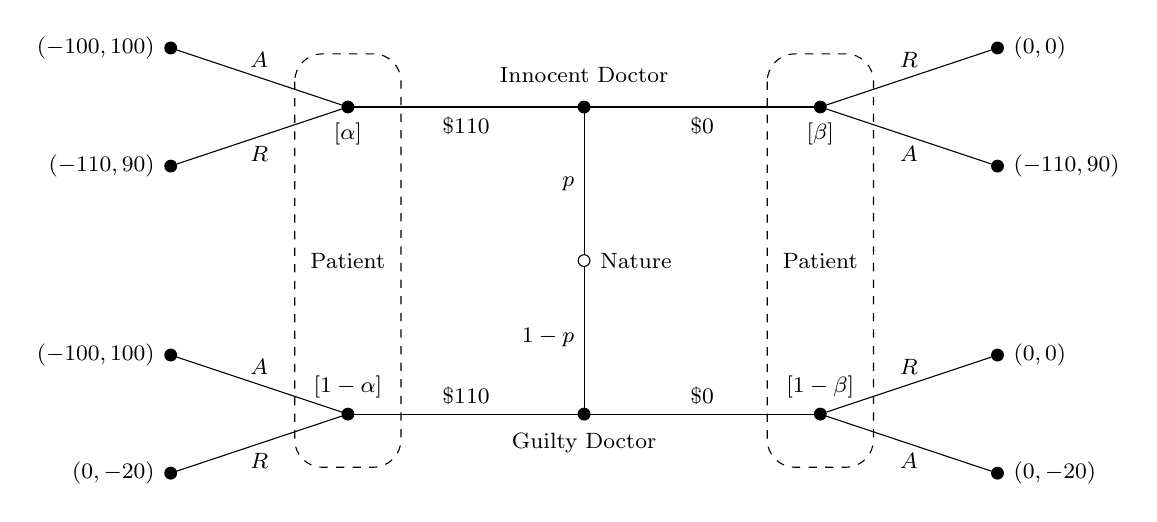
\begin{tikzpicture}[scale=1.5,font=\footnotesize]
\tikzset{S/.style={circle,draw,inner sep=1.5,fill=black},
H/.style={circle,draw,inner sep=1.5}
}


% Specify spacing for each level of the tree

\tikzstyle{level 1}=[level distance=13mm,sibling distance=30mm]

\tikzstyle{level 2}=[level distance=20mm,sibling distance=20mm]

\tikzstyle{level 3}=[level distance=15mm,sibling distance=10mm]

% The Tree
\node(0)[H,label=right:{Nature}]{}

child[grow=up]{node[S,label=above:{\begin{tabular}{c}
%Top level label
Innocent Doctor\\
\end{tabular}}] {}
child[grow=left]{node(1)[S,label=below:{$[\alpha]$}]{}
child{node[S,label=left:{$(-100,100)$}]{} edge from parent node [above]{$A$}}
child{node[S,label=left:{$(-110,90)$}]{} edge from parent node [below]{$R$}}
edge from parent node [below]{$\$ 110$} 
}
child[grow=right]{node(3)[S,label=below:{$[\beta]$}]{}
child{node[S,label=right:{$(-110,90)$}]{} edge from parent node [below]{$A$}}
child{node[S,label=right:{$(0,0)$}]{} edge from parent node [above]{$R$}}
edge from parent node [below]{$\$0$}
}
%Percentage top
edge from parent node [left]{$p$}
}
child[grow=down]{node[S,label=below:{\begin{tabular}{c}
%Bottom level label
Guilty Doctor\\
\end{tabular}}] {}
child[grow=left]{node(2)[S,label=above:{$[1-\alpha]$}]{}
child{node[S,label=left:{$(-100,100)$}]{} edge from parent node [above]{$A$}}
child{node[S,label=left:{$(0,-20)$}]{} edge from parent node [below]{$R$}}
edge from parent node [above]{$\$110$}
}
child[grow=right]{node(4)[S,label=above:{$[1-\beta]$}]{}
child{node[S,label=right:{$(0,-20)$}]{} edge from parent node [below]{$A$}}
child{node[S,label=right:{$(0,0)$}]{} edge from parent node [above]{$R$}}
edge from parent node [above]{$\$ 0$}
}
%Percentage down
edge from parent node [left]{$1-p$}
};


% information set

\draw[dashed,rounded corners=10]($(1) + (-.45,.45)$)rectangle($(2) +(.45,-.45)$);
\draw[dashed,rounded corners=10]($(3) + (-.45,.45)$)rectangle($(4) +(.45,-.45)$);

% specify mover at 2nd information set

\node at ($(1)!.5!(2)$) {Patient};

\node at ($(3)!.5!(4)$) {Patient};

\end{tikzpicture}
\end{center}
\end{document}